Em uma análise de como os passos seriam sequenciados de uma maneira mais clara e simplificada, as atividades de envio e recebimento de mensagens acerca do status da solicitação foram substituídas por uma atividade de consulta de dados realizada pela própria empresa. 
\\ \indent Imaginando que cabe à empresa a decisão sobre corrigir os erros ou desistir da participação, foi criada uma atividade onde a viabilidade da correção dos erros é colocada em pauta, com um gateway que indica qual a decisão tomada.
\\ \indent A Figura \ref{fig:atividaderemovidadois} apresenta a remoção das atividades relacionadas a envio e recebimento de mensagem sobre o status do AS-IS para criação do TO-BE.
\begin{figure}[H]
	\centering
	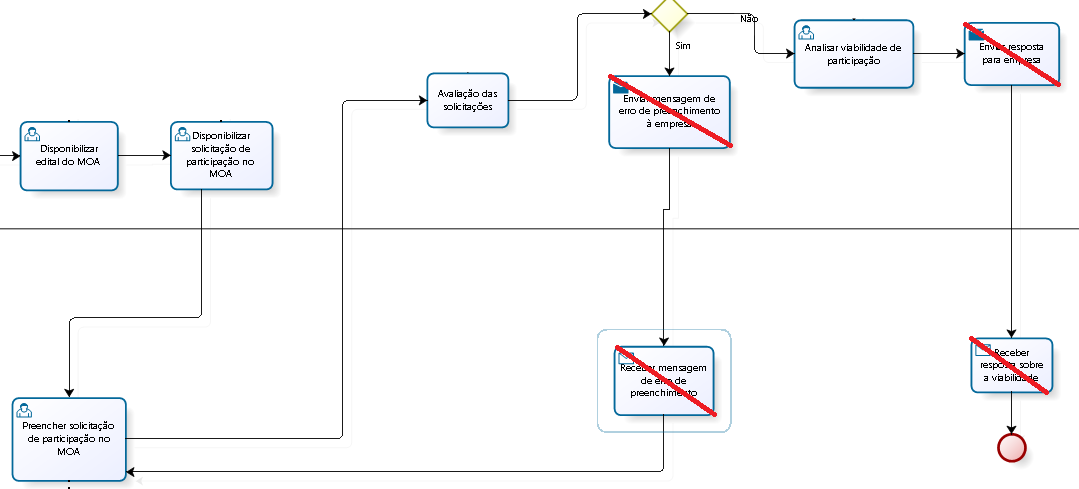
\includegraphics[scale=0.5]{remover_atividades_2}
	\caption[Atividades Removidas pelo Critério de Simplificação]{Atividades Removidas pelo Critério de Simplificação.}
	\label{fig:atividaderemovidadois}
\end{figure}
A Figura \ref{fig:atividaderemovidatres} apresenta a inclusão de atividades desenvolvidas pelas empresas solicitantes que melhoram e simplificam o sequenciamento das atividades logo após análise da viabilidade da participação da empresa pela CHAMEX:
\begin{figure}[H]
	\centering
	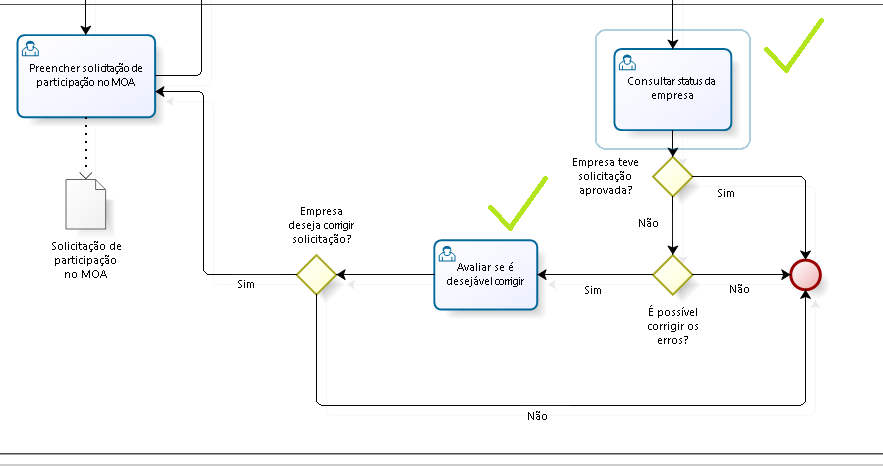
\includegraphics[scale=0.6]{remover_atividades_3}
	\caption[Inclusão de Atividades pelo Critério de Melhoria de Sequenciamento]{Inclusão de Atividades pelo Critério de Melhoria de Sequenciamento.}
	\label{fig:atividaderemovidatres}
\end{figure}